\begin{savequote}[45mm]
\ascii{Any fool can write code that a computer can understand. Good programmers write code that humans can understand.}
\qauthor{\ascii{- Martin Flower}}
\end{savequote}

\chapter{C API:分水岭} 
\label{ch:c-api}

\begin{content}

本章通过客户端\ascii{Session}生命周期的实现为例,揭示前端\ascii{Python}与后端\cpp{}系统的实现通道,揭示\ascii{TensorFlow}多语言编程的奥秘。

\end{content}

\section{Swig:幕后英雄}

\begin{content}

前端多语言编程环境与后端\cpp{}实现系统的通道归功于\ascii{Swig}的包装器。\ascii{TensorFlow}使用\ascii{Bazel}的构建工具,在系统编译之前启动\ascii{Swig}的代码生成过程,通过\code{tensorflow.i}自动生成了两个适配(\ascii{Wrapper})文件:

\begin{enum}
  \eitem{\code{pywrap\_tensorflow.py}:  负责对接上层\ascii{Python}调用;}
  \eitem{\code{pywrap\_tensorflow.cpp}: 负责对接下层\ascii{C API}调用。}
\end{enum}

\code{pywrap\_tensorflow.py}模块首次被导入时,自动地加载\code{\_pywrap\_tensorflow.so}的动态链接库。从而在运行时实现了\code{pywrap\_tensorflow.py}到\code{pywrap\_tensorflow.cpp}的函数调用关系。

如\refig{swig}所示,在\code{pywrap\_tensorflow.cpp}的实现中,静态注册了一个函数符号表,实现了\ascii{Python}函数名到\ascii{C}函数名的二元关系。在运行时,按照\ascii{Python}的函数名称,匹配找到对应的\ascii{C}函数实现,最终实现到\code{c\_api.c}具体实现的调用关系。

\begin{figure}[H]
\centering
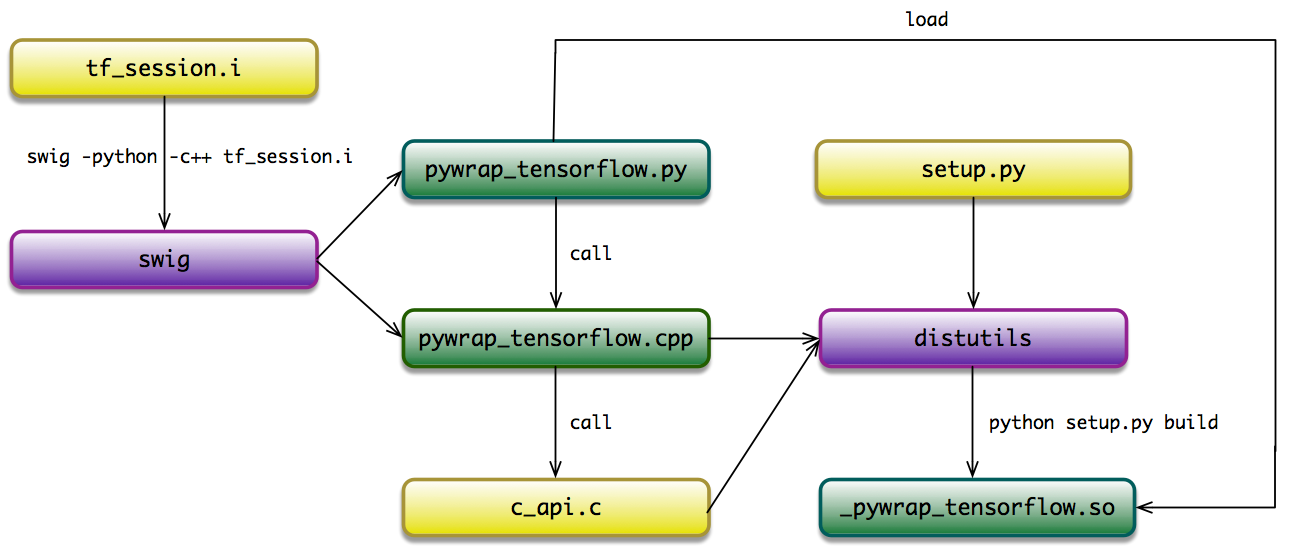
\includegraphics[width=0.9\textwidth]{figures/swig.png}
\caption{Swig代码生成器}}
 \label{fig:swig}
\end{figure}

下文以客户端\ascii{Session}生命周期的实现为例,揭示前端\ascii{Python}与后端\cpp{}系统的实现通道。

\end{content}

\section{客户端代理}

\begin{content}

在上一章提及,\ascii{C API}并非是\ascii{Client}与\ascii{Master}的分界线。如\refig{tf-client-session}所示,\ascii{Client}存在部分\cpp{}实现,即\code{tensorflow::Session}。其中,\code{tf.Session}实例直接持有\code{tensorflow::Session}实例的句柄。

在真实运行时环境中,\code{tensorflow::Session}可能存在多种实现。例如,\code{tensorflow::DirectSession}负责\emph{本地模式}的会话控制。而\code{tensorflow::GrpcSession}负责基于\ascii{gRPC}协议的\emph{分布式模式}的会话控制。

一般地,用户使用的是\code{tf.Session}编程,而非\code{tensorflow::Session}。因此,后者常常称为前者的代理实现。

\begin{figure}[!h]
\centering
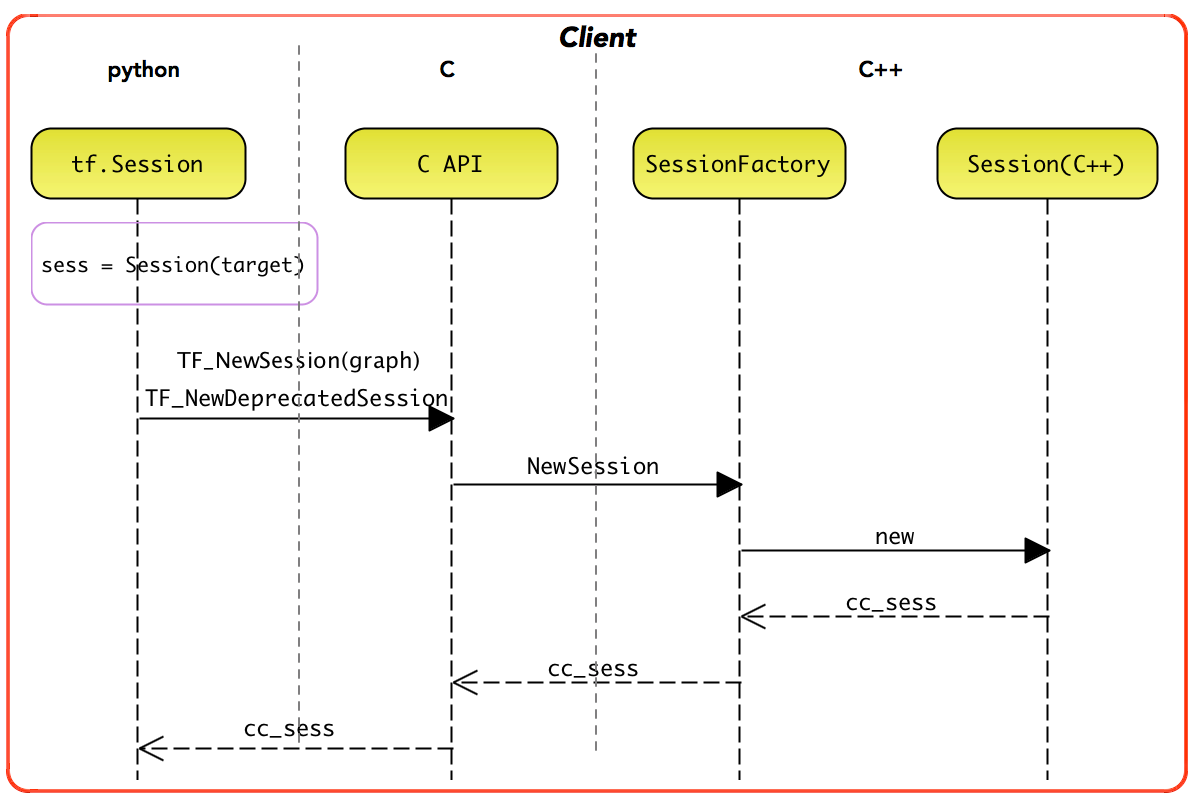
\includegraphics[width=0.9\textwidth]{figures/tf-client-session.png}
\caption{客户端:tensorflow::Session实例创建过程}}
 \label{fig:tf-client-session}
\end{figure}

\end{content}

\section{会话生命周期}

\begin{content}

会话的生命周期包括会话的创建,加载计算图,扩展计算图,执行计算图,关闭会话,销毁会话的基本过程。在前端\ascii{Python}和后端\cpp{}表现为两套相兼容的接口实现。

\subsection{Python前端}

在\ascii{Python}前端,\code{Session}的生命周期主要体现在:

\begin{enum}
  \eitem{创建\code{Session(target)};}
  \eitem{迭代执行\code{Session.run(fetches, feed\_dict)};}
    \begin{enum}
      \eitem{\code{Session.\_extend\_graph(graph)};}
      \eitem{\code{Session.TF\_Run(feeds, fetches, targets)};}
    \end{enum}
  \eitem{关闭\code{Session};}
  \eitem{销毁\code{Session};}
\end{enum}

\begin{figure}[!htbp]
\centering
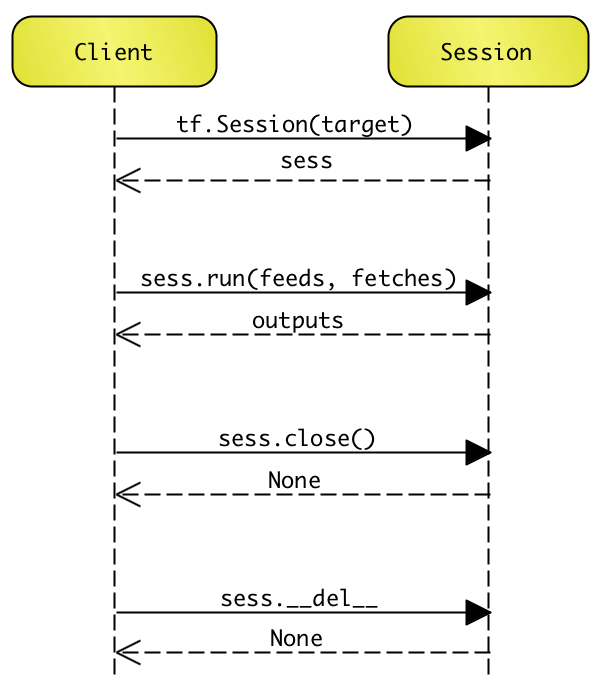
\includegraphics[width=0.7\textwidth]{figures/py-session-lifecycle.png}
\caption{Python: Session生命周期}}
 \label{fig:py-session-lifecycle}
\end{figure}

例如,此处创建了本地模式的\code{Session}实例,并启动\code{mnist}的训练过程。

\begin{leftbar}
\begin{python}
sess = tf.Session()
for _ in range(1000):
  batch_xs, batch_ys = mnist.train.next_batch(100)
  sess.run(train_step, feed_dict={x: batch_xs, y_: batch_ys})
sess.close()
\end{python}
\end{leftbar}

\subsection{C++后端}

相应地,在\cpp{}后端,\code{Session}的生命周期主要体现在:

\begin{enum}
  \eitem{根据\code{target}多态创建\code{Session};}
  \eitem{\code{Session.Create(graph)}:有且仅有一次;}
  \eitem{\code{Session.Extend(graph)}:零次或多次;}
  \eitem{迭代执行\code{Session.Run(inputs, outputs, targets)};}
  \eitem{关闭\code{Session.Close};}
  \eitem{销毁\code{Session}对象。}
\end{enum}

\begin{figure}[!htbp]
\centering
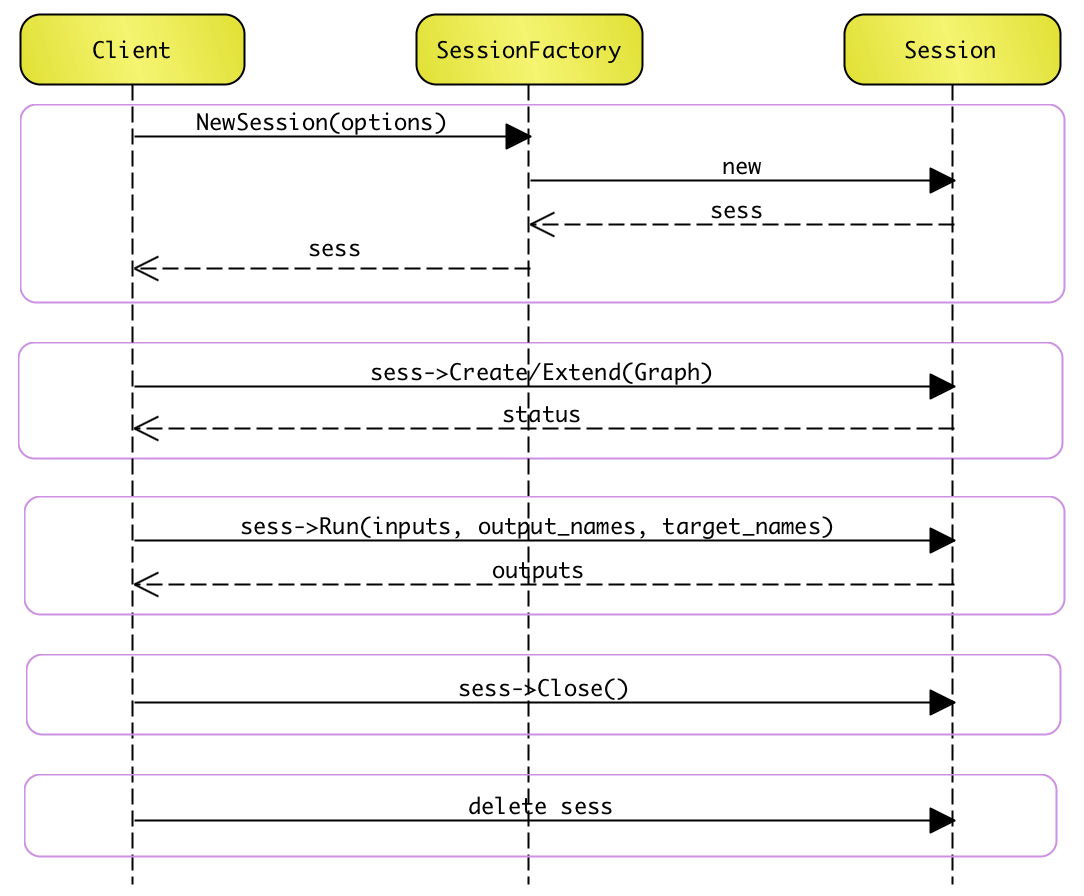
\includegraphics[width=0.9\textwidth]{figures/cc-session-lifecycle.png}
\caption{C++: Session生命周期}}
 \label{fig:cc-session-lifecycle}
\end{figure}

例如,此处创建了本地模式的\code{DirectSession}实例,并启动计算图的执行过程。

\begin{leftbar}
\begin{c++}
// create/load graph ...
tensorflow::GraphDef graph;

// local runtime, target is ""
tensorflow::SessionOptions options;

// create Session
std::unique_ptr<tensorflow::Session> 
sess(tensorflow::NewSession(options));

// create graph at initialization.
tensorflow::Status s = sess->Create(graph);
if (!s.ok()) { ... }

// run step
std::vector<tensorflow::Tensor> outputs;
s = session->Run(
  {},               // inputs is empty
  {"output:0"},     // outputs names
  {"update_state"}, // target names
  &outputs);        // output tensors
if (!s.ok()) { ... }

// close
session->Close();
\end{c++}
\end{leftbar}

\end{content}

\section{创建会话}

\begin{content}

下面介绍Session创建的详细过程,从\ascii{Python}前端为起点,通过Swig自动生成的\ascii{Python-C++}的包装器为媒介,实现了\ascii{Python}到\ascii{TensorFlow}的\ascii{C API}的调用。

其中,\ascii{C API}是前端系统与后端系统的分水岭。后端\cpp{}系统根据前端传递的\code{Session.target},使用\code{SessionFactory}多态创建\code{tensorflow::Session}对象。

\begin{figure}[!h]
\centering
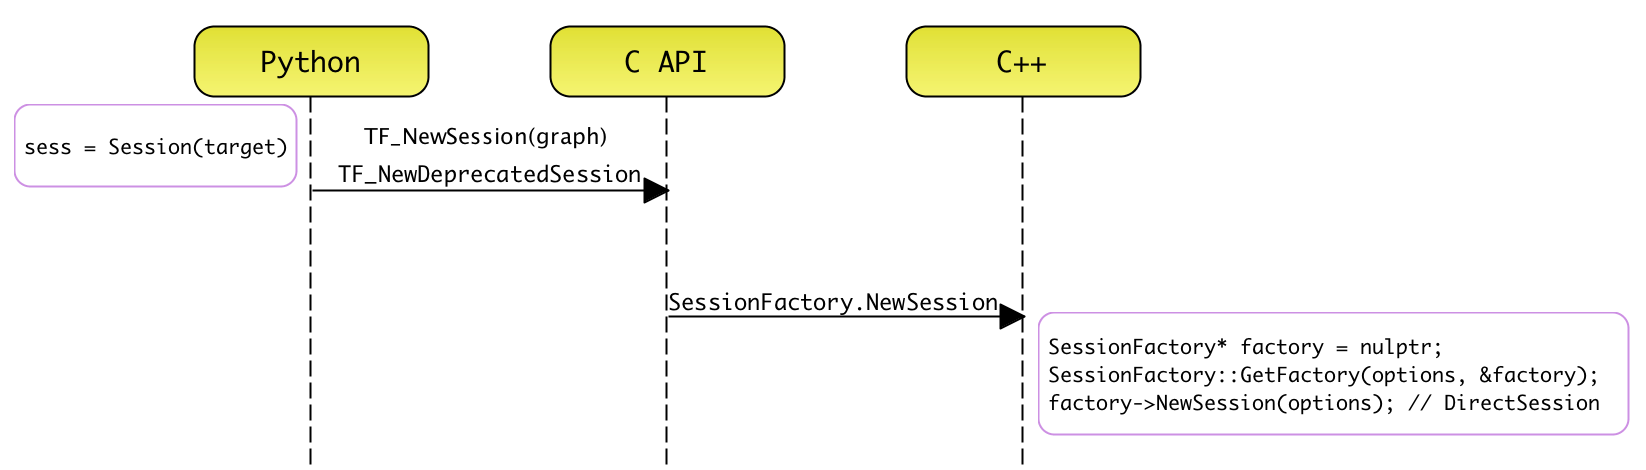
\includegraphics[width=1.0\textwidth]{figures/py-create-session.png}
\caption{创建会话}}
 \label{fig:py-create-session}
\end{figure}

\subsection{编程接口}

当\ascii{Client}要启动计算图的执行过程时,先创建了一个\code{Session}实例,进而调用父类\code{BaseSession}的构造函数。

\begin{leftbar}
\begin{python}
# tensorflow/python/client/session.py
class Session(BaseSession):
  def __init__(self, target='', graph=None, config=None):
    super(Session, self).__init__(target, graph, config=config)
    # ignoring implements...
\end{python}
\end{leftbar}

在\code{BaseSession}的构造函数中,将调用\code{pywrap\_tensorflow}模块中的函数。其中,\code{pywrap\_tensorflow}模块自动由\ascii{Swig}生成。

\begin{leftbar}
\begin{python}
# tensorflow/python/client/session.py
from tensorflow.python import pywrap_tensorflow as tf_session

class BaseSession(SessionInterface):
  def __init__(self, target='', graph=None, config=None):
    # ignoring implements...
    with errors.raise_exception_on_not_ok_status() as status:
        self._session = tf_session.TF_NewDeprecatedSession(opts, status)
\end{python}
\end{leftbar}

\subsubsection{Python包装器}

在\code{pywrap\_tensorflow}模块中,通过\code{\_pywrap\_tensorflow}的转发,实现了从\ascii{Python}到动态连接库\code{\_pywrap\_tensorflow.so}中调用对应的\cpp{}函数实现。

\begin{leftbar}
\begin{python}
# tensorflow/bazel-bin/tensorflow/python/pywrap\_tensorflow.py
def TF_NewDeprecatedSession(opts, status):
    return _pywrap_tensorflow.TF_NewDeprecatedSession(opts, status)
\end{python}
\end{leftbar}

\subsubsection{C++包装器}

在\code{pywrap\_tensorflow.cpp}的具体实现中,静态注册了函数调用的符号表,实现\ascii{Python}的函数名称到\cpp{}函数实现的具体映射。

\begin{leftbar}
\begin{c++}
// tensorflow/bazel-bin/tensorflow/python/pywrap\_tensorflow.cpp
static PyMethodDef SwigMethods[] = {
   // ...
  { "TF_NewDeprecatedSession", 
    _wrap_TF_NewDeprecatedSession, METH_VARARGS, NULL},
};
\end{c++}
\end{leftbar}

最终,\code{\_wrap\_TF\_NewDeprecatedSession}将调用\code{c\_api.h}对其开放的\ascii{API}接口:\code{TF\_NewDeprecatedSession}。也就是说,自动生成的\code{pywrap\_tensorflow.cpp}仅仅负责\ascii{Python}函数到\ascii{C/C++}函数调用的转发,最终将调用底层\ascii{C}系统向上提供的\ascii{API}接口。

\subsection{C API}

\code{c\_api.h}是\ascii{TensorFlow}的后端执行系统面向前端开放的公共\ascii{API}接口。

\begin{leftbar}
\begin{c++}
// tensorflow/c/c\_api.c
TF_DeprecatedSession* TF_NewDeprecatedSession(
  const TF_SessionOptions* opt, TF_Status* status) {
  Session* session;
  status->status = NewSession(opt->options, &session);
  return status->status.ok() ? new TF_DeprecatedSession({session}) : NULL;
}
\end{c++}
\end{leftbar}

\subsection{后端系统}

\code{NewSession}将根据前端传递的\code{Session.target},使用\code{SessionFactory}多态创建不同类型的\code{tensorflow::Session}对象。

\begin{leftbar}
\begin{c++}
Status NewSession(const SessionOptions& options, Session** out_session) {
  SessionFactory* factory;
  Status s = SessionFactory::GetFactory(options, &factory);
  if (!s.ok()) {
    *out_session = nullptr;
    return s;
  }
  *out_session = factory->NewSession(options);
  if (!*out_session) {
    return errors::Internal("Failed to create session.");
  }
  return Status::OK();
}
\end{c++}
\end{leftbar}

\subsubsection{工厂方法}

在后端\cpp{}系统中,\code{tensorflow::Session}的创建使用了抽象工厂方法。如果\code{SessionOptions}中的\code{target}为空字符串(默认的),则创建\code{DirectSession}实例,启动本地运行模式;如果\code{SessionOptions}中的\code{target}为\code{grpc}开头,则创建\code{GrpcSession}实例,启动基于\code{RPC}的分布式运行模式。如\refig{cc-session-factory}所示。

\begin{figure}[!h]
\centering
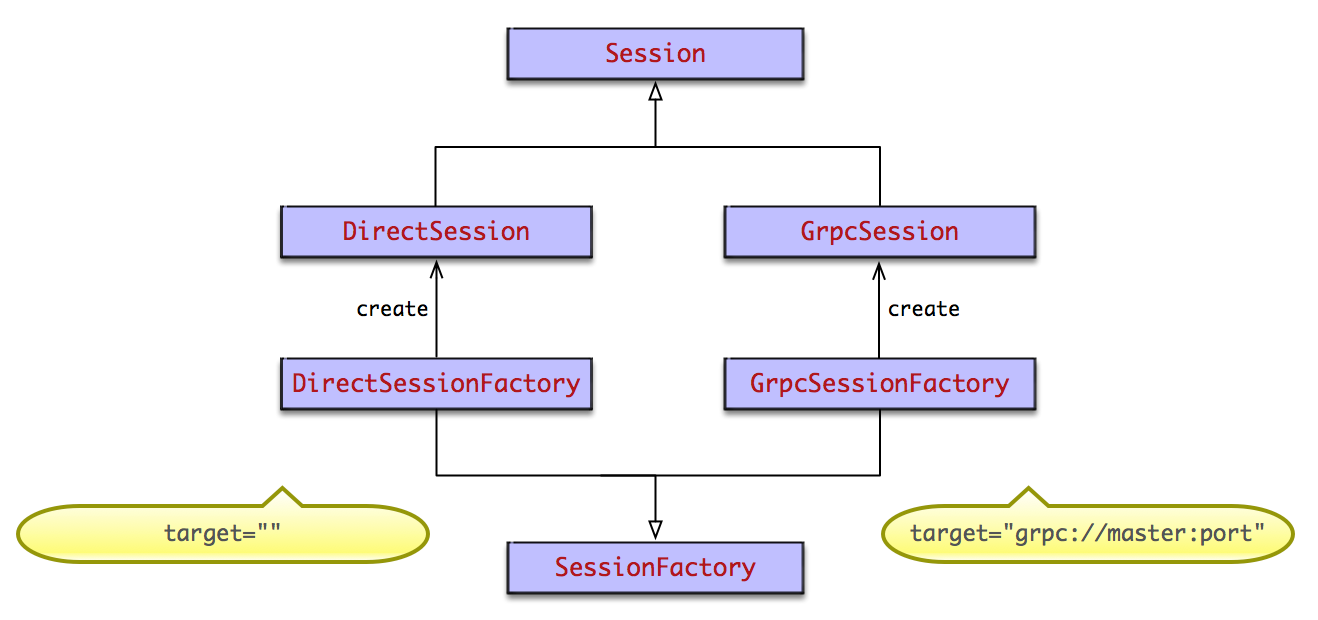
\includegraphics[width=0.9\textwidth]{figures/cc-session-factory.png}
\caption{tensorflow::Session创建:抽象工厂方法}}
 \label{fig:cc-session-factory}
\end{figure}

\end{content}

\section{创建/扩展图}

\begin{content}

随后,\ascii{Python}前端将迭代调用\code{Session.run}接口,将构造好的计算图,以\code{GraphDef}的形式发送给\cpp{}后端。

其中,前端每次调用\code{Session.run}接口时,都会试图将新增节点的计算图发送给后端系统,以便将新增节点的计算图\ascii{Extend}到原来的计算图中。特殊地,在首次调用\code{Session.run}时,将发送整个计算图给后端系统。

后端系统首次调用\code{Session.Extend}时,转调(或等价实现)\code{Session.Create};以后,后端系统每次调用\code{Session.Extend}时将真正执行\code{Extend}的语义,将新增的计算图的节点追加至原来的计算图中。

\begin{figure}[!htbp]
\centering
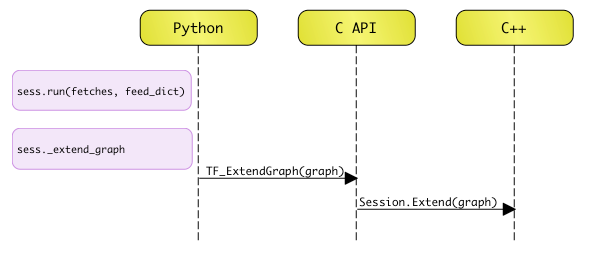
\includegraphics[width=0.9\textwidth]{figures/py-session-create-graph.png}
\caption{创建图}}
 \label{fig:py-session-create-graph}
\end{figure}

\subsection{编程接口}

\begin{leftbar}
\begin{python}
# tensorflow/python/client/session.py
class Session(BaseSession):
  def run(self, fetch_list, feed_dict=None, options=None, run_metadata=None):
    # ignores implements...
    self._extend_graph()
    with errors.raise_exception_on_not_ok_status() as status:
      return tf_session.TF_Run(
        self, options, feeds, fetches, targets, status, run_metadata)
\end{python}
\end{leftbar}

其中,在首次调用\code{self.\_extend\_graph}时,或者有新的节点被添加至计算图中时,对计算图\code{GraphDef}实施序列化操作,最终触发\code{tf\_session.TF\_ExtendGraph}的调用。

\begin{leftbar}
\begin{python}
from tensorflow.python import pywrap_tensorflow as tf_session

class Session(BaseSession):
  def _extend_graph(self):
    # ignores implements...
    with errors.raise_exception_on_not_ok_status() as status:
      tf_session.TF_ExtendGraph(
        self._session, graph_def.SerializeToString(), status)
\end{python}
\end{leftbar}

\subsubsection{Python包装器}

\begin{leftbar}
\begin{python}
# tensorflow/bazel-bin/tensorflow/python/pywrap\_tensorflow.py
def TF_ExtendGraph(sess, graph_def, status):
  return _pywrap_tensorflow.TF_ExtendGraph(sess, graph_def, status)
\end{python}
\end{leftbar}

\subsubsection{C++包装器}

\begin{leftbar}
\begin{c++}
// tensorflow/bazel-bin/tensorflow/python/pywrap\_tensorflow.cpp
static PyMethodDef SwigMethods[] = {
  // ignore implements...
  { (char *)"TF_ExtendGraph", _wrap_TF_ExtendGraph, METH_VARARGS, NULL},
};
\end{c++}
\end{leftbar}

\subsection{C API}

\code{TF\_ExtendGraph}是\ascii{C API}对接上层编程环境的接口;首先,它完成计算图\code{GraphDef}的反序列化,最终调用\code{tensorflow::Session}的\code{Extend}接口。

\begin{leftbar}
\begin{c++}
// tensorflow/c/c\_api.c
void TF_ExtendGraph(TF_DeprecatedSession* sess, 
  const void* proto, size_t proto_len, TF_Status* status) {
  GraphDef g;
  if (!tensorflow::ParseProtoUnlimited(&g, proto, proto_len)) {
    status->status = InvalidArgument("Invalid GraphDef");
    return;
  }
  status->status = sess->session->Extend(g);
}
\end{c++}
\end{leftbar}

\subsection{后端系统}

\code{tensorflow::Session}在运行时根据\code{Session}的动态类型,将多态地调用相应子类的实现。

\begin{leftbar}
\begin{c++}
class Session {
public:
  virtual Status Create(const GraphDef& graph) = 0;
  virtual Status Extend(const GraphDef& graph) = 0;
};
\end{c++}
\end{leftbar}

其中,\code{Create}表示在当前的\code{tensorflow::Session}实例上注册计算图,如果要注册新的计算图,需要关闭该\code{tensorflow::Session}对象。\code{Extend}表示在\code{tensorflow::Session}实例上已注册的计算图上追加节点。

\code{Extend}首次执行时,等价于\code{Create}的语义;因为首次\code{Extend}时,已注册的计算图为空。事实上,系统就是按照如上方案实现的,此处以\code{GrpcSession}实现为例。

\subsubsection{首次扩展图: GrpcSession}

首先,如果判断引用\code{Master}的\code{handle}不为空,则执行\code{Extend};否则,执行\code{Create}的语义,建立与\code{Master}的连接,并持有\code{Master}的\code{handle}。

\begin{leftbar}
\begin{c++}
Status GrpcSession::Extend(const GraphDef& graph) {
  CallOptions call_options;
  call_options.SetTimeout(options_.config.operation_timeout_in_ms());
  return ExtendImpl(&call_options, graph);
}

Status GrpcSession::ExtendImpl
  (CallOptions* call_options, const GraphDef& graph) {
  if (handle_is_empty()) {
    // Session was unitialized, 
    // so simply initialize the session with 'graph'.
    return Create(graph);
  }
  // ignore implements...  
}
\end{c++}
\end{leftbar}

\end{content}

\section{迭代运行}

\begin{content}

接着,\ascii{Python}前端\code{Session.run}实现将\code{fetches, feed\_dict}传递给后端系统。后端系统调用\code{Session.Run}接口。

后端系统的一次\code{Session.Run}执行常常被称为一次\ascii{Step}。其中,\ascii{Step}的执行过程是\ascii{TensorFlow}运行时的关键路径。

每次\ascii{Step},计算图将正向计算网络的输出,然后反向传递梯度,并完成一次训练参数的更新。首先,后端系统根据\ascii{fetches, targets},对计算图(常称为\ascii{Full Graph})进行剪枝,得到一个最小依赖的子图(常称为\ascii{Client Graph})。

然后,运行时启动设备分配算法,如果节点之间的边横跨设备,则将该边分裂,插入相应的\code{Send}与\code{Recv}节点,实现跨设备节点的通信机制。

随后,将分裂出来的子图片段(常称为\ascii{Graph Partition})注册到相应的\ascii{Worker}上,并启动各个\ascii{Worker}并发执行这些子图片段。如\refig{py-session-run}所示。

\begin{figure}[!h]
\centering
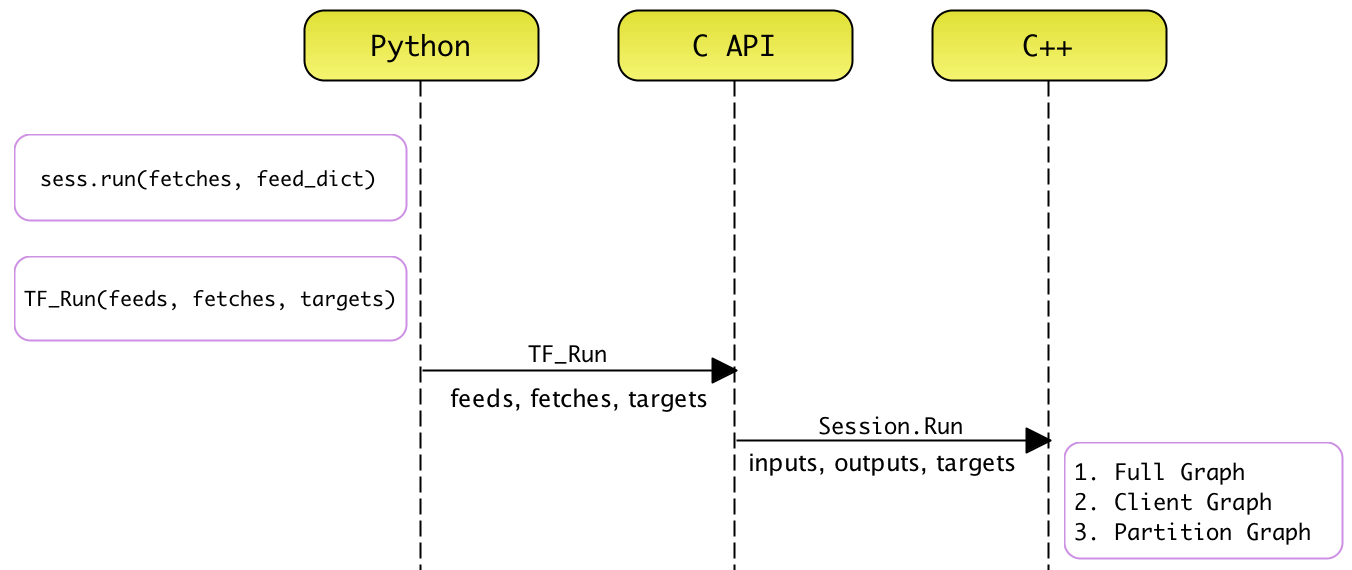
\includegraphics[width=0.9\textwidth]{figures/py-session-run.png}
\caption{迭代执行}}
 \label{fig:py-session-run}
\end{figure}

\subsection{编程接口}

当\ascii{Client}调用\ascii{Session.run}时,最终会调用\ascii{pywrap\_tensorflow}模块中的函数。

\begin{leftbar}
\begin{python}
# tensorflow/python/client/session.py
from tensorflow.python import pywrap_tensorflow as tf_session

class Session(BaseSession):
  def run(self, fetch_list, feed_dict=None, options=None, run_metadata=None):
    # ignores other implements...
    self._extend_graph()
    with errors.raise_exception_on_not_ok_status() as status:
      return tf_session.TF_Run(
        self, options, feeds, fetches, targets, status, run_metadata)
    # ignores other implements...
\end{python}
\end{leftbar}

\subsubsection{Python包装器}

\begin{leftbar}
\begin{python}
# tensorflow/bazel-bin/tensorflow/python/pywrap\_tensorflow.py
def TF_Run(sess, options, feeds, outputs, targets, status, run_metadata):
  return _pywrap_tensorflow.TF_Run(
    sess, options, feeds, outputs, targets, status, run_metadata)
\end{python}
\end{leftbar}

\subsubsection{C++包装器}

\begin{leftbar}
\begin{c++}
// tensorflow/bazel-bin/tensorflow/python/pywrap\_tensorflow.cpp
static PyMethodDef SwigMethods[] = {
  // ...
  { (char *)"TF_Run", _wrap_TF_Run, METH_VARARGS, NULL},
};
\end{c++}
\end{leftbar}

最终,\code{\_wrap\_TF\_Run}将转调\ascii{C API}对应的\code{TF\_Run}接口函数。

\subsection{C API}

\code{TF\_Run}是\ascii{C API}对接上层编程环境的接口。首先,它完成输入数据从\ascii{C}到\cpp{}的格式转换,并启动后台的\code{tensorflow::Session}的执行过程;当执行完成后,再将\code{outputs}的输出数据从\cpp{}到\ascii{C}的格式转换。

\begin{leftbar}
\begin{c++}
// tensorflow/c/c\_api.c
void TF_Run(TF_DeprecatedSession* s, 
  // session options
  const TF_Buffer* run_options,
  // Input tensors
  const char** c_input_names, TF_Tensor** c_inputs, int ninputs,
  // Output tensors
  const char** c_output_names, TF_Tensor** c_outputs, int noutputs,
  // Target nodes
  const char** c_target_oper_names, int ntargets,
  // run\_metadata
  TF_Buffer* run_metadata, TF_Status* status) {
  // convert data format, ignore implements...
  s->session->Run(options_proto, input_names, output_names,
                  target_names, &outputs, &run_metadata); 
  // store results in c\_outputs...
}
\end{c++}
\end{leftbar}

\subsection{后端系统}

\code{tensorflow::Session}在运行时其动态类型,将多态地调用相应的子类实现。

\begin{leftbar}
\begin{c++}
class Session {
public:
  virtual Status Run(
    const RunOptions& options,
    const vector<pair<string, Tensor> >& inputs,
    const vector<string>& output_names,
    const vector<string>& target_names,
    vector<Tensor>* outputs, RunMetadata* run_metadata) {
      return errors::Unimplemented(
        "Run with options is not supported for this session.");
  }
};
\end{c++}
\end{leftbar}

输入包括:

\begin{enum}
  \eitem{\code{options}:\code{Session}的运行配置参数;}
  \eitem{\code{inputs}: 输入\code{Tensor}的名字列表;}
  \eitem{\code{output\_names}: 输出\code{Tensor}的名字列表;}
  \eitem{\code{targets}: 无输出,待执行的\ascii{OP}的名字列表。} 
\end{enum}

输出包括:

\begin{enum}
  \eitem{\code{outputs}: 输出的\code{Tensor}列表;}
  \eitem{\code{run\_metadata}: 运行时元数据的收集器。}
\end{enum}

其中,输出的\code{outputs}列表与输入的\code{output\_names}一一对应,如果运行时因并发执行,导致\code{outputs}乱序执行,最终返回时需要对照输入的\code{output\_names}名字列表,对\code{outputs}进行排序。

\end{content}

\section{关闭会话}

\begin{content}

当计算图执行完毕后,需要关闭\code{tf.Session},以便释放后端的系统资源,包括队列,\ascii{IO}等。会话关闭流程较为简单,如\refig{py-session-close}所示。。

\begin{figure}[!h]
\centering
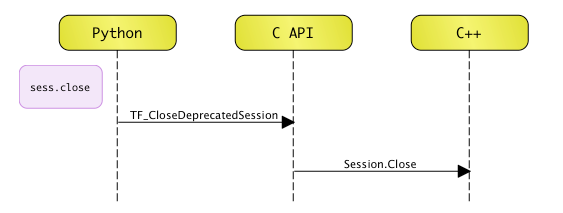
\includegraphics[width=0.9\textwidth]{figures/py-session-close.png}
\caption{关闭会话}}
 \label{fig:py-session-close}
\end{figure}

\subsection{编程接口}

当\ascii{Client}调用\code{Session.close}时,最终会调用\code{pywrap\_tensorflow}模块中的函数: \code{TF\_CloseDeprecatedSession}。

\begin{leftbar}
\begin{python}
# tensorflow/python/client/session.py
from tensorflow.python import pywrap_tensorflow as tf_session

class Session(BaseSession):
  def close(self):
    # ignores other implements...
    with errors.raise_exception_on_not_ok_status() as status:
      tf_session.TF_CloseDeprecatedSession(self._session, status)
\end{python}
\end{leftbar}

\subsubsection{Python包装器}

\begin{leftbar}
\begin{python}
# tensorflow/bazel-bin/tensorflow/python/pywrap\_tensorflow.py
def TF_CloseDeprecatedSession(sess, status):
  return _pywrap_tensorflow.TF_CloseDeprecatedSession(sess, status)
\end{python}
\end{leftbar}

\subsubsection{C++包装器}

\begin{leftbar}
\begin{c++}
// tensorflow/bazel-bin/tensorflow/python/pywrap\_tensorflow.cpp
static PyMethodDef SwigMethods[] = {
  // ...
  { (char *)"TF_CloseDeprecatedSession", 
    _wrap_TF_CloseDeprecatedSession, METH_VARARGS, NULL},
};
\end{c++}
\end{leftbar}

最终,\code{\_wrap\_TF\_CloseDeprecatedSession}将转调\ascii{C API}对应的\code{TF\_CloseDeprecatedSession}接口函数。

\subsection{C API}

\code{TF\_CloseDeprecatedSession}直接完成\code{tensorflow::Session}的关闭操作。

\begin{leftbar}
\begin{c++}
void TF_CloseDeprecatedSession(TF_DeprecatedSession* s, TF_Status* status) {
  status->status = s->session->Close();
}
\end{c++}
\end{leftbar}

\subsection{后端系统}

\code{Session(C++)}在运行时其动态类型,将多态地调用相应的子类实现。

\begin{leftbar}
\begin{c++}
class Session {
public:
  virtual Status Close() = 0;
};
\end{c++}
\end{leftbar}

\end{content}

\section{销毁会话}

\begin{content}

当\code{tf.Session}不在被使用,由\ascii{Python}的\ascii{GC}释放。\code{Session.\_\_del\_\_}被调用后,将启动后台\code{tensorflow::Session}对象的析构过程。如\refig{py-delete-session}所示。

\begin{figure}[!h]
\centering
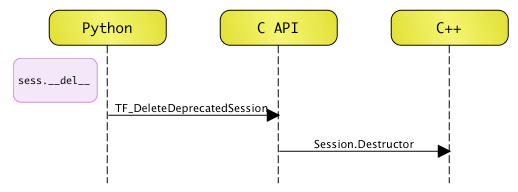
\includegraphics[width=0.9\textwidth]{figures/py-delete-session.png}
\caption{销毁会话}
 \label{fig:py-delete-session}
\end{figure}

\subsection{编程接口}

当\ascii{Client}调用\code{Session.\_\_del\_\_}时,先启动\code{Session.close}的调用,最终会调用\code{pywrap\_tensorflow}模块中的函数: \code{TF\_DeleteDeprecatedSession}。

\begin{leftbar}
\begin{python}
# tensorflow/python/client/session.py
from tensorflow.python import pywrap_tensorflow as tf_session

class Session(BaseSession):
  def __del__(self):
    # 1. close session unconditionally.
    try:
      self.close()
    except Exception:
      pass
    # 2. delete session unconditionally.
    if self._session is not None:
      try:
        status = tf_session.TF_NewStatus()
        tf_session.TF_DeleteDeprecatedSession(self._session, status)
      finally:
        tf_session.TF_DeleteStatus(status)
      self._session = None
\end{python}
\end{leftbar}

\subsubsection{Python包装器}

\begin{leftbar}
\begin{python}
# tensorflow/bazel-bin/tensorflow/python/pywrap\_tensorflow.py
def TF_DeleteDeprecatedSession(sess, status):
  return _pywrap_tensorflow.TF_DeleteDeprecatedSession(sess, status)
\end{python}
\end{leftbar}

\subsubsection{C++包装器}

\begin{leftbar}
\begin{c++}
// tensorflow/bazel-bin/tensorflow/python/pywrap\_tensorflow.cpp
static PyMethodDef SwigMethods[] = {
  // ...
  { (char *)"TF_DeleteDeprecatedSession", 
    _wrap_TF_DeleteDeprecatedSession, METH_VARARGS, NULL},
};
\end{c++}
\end{leftbar}

最终,\code{\_wrap\_TF\_DeleteDeprecatedSession}将转调\ascii{C API}对应的\code{TF\_DeleteDeprecatedSession}接口函数。

\subsection{C API}

\code{TF\_DeleteDeprecatedSession}直接完成\code{Session(C++)}对象的释放。

\begin{leftbar}
\begin{c++}
void TF_DeleteDeprecatedSession(TF_DeprecatedSession* s, TF_Status* status) {
  status->status = Status::OK();
  delete s->session;
  delete s;
}
\end{c++}
\end{leftbar}

\subsection{后端系统}

\code{tensorflow::Session}在运行时其动态类型,多态地调用相应子类实现的析构函数。

\begin{leftbar}
\begin{c++}
class Session {
public:
  virtual ~Session() {};
};
\end{c++}
\end{leftbar}

\end{content}

\section{性能调优}

\begin{content}

一般地,一个\code{Session}只能运行一个计算图。如果一个\code{Session}要运行其他的计算图,必须先关掉\code{Session},然后再将新图注册到此\code{Session}中,最后启动新的计算图的执行过程。

事实上,一个计算图可以运行在多个\code{Session}实例上。如果在\code{Graph}实例上维持\code{Session}的引用计数器,在\code{Session}创建时,在该图实例上增加\ascii{1};在\code{Session}销毁时(不是关闭\code{Session}),在该图实例上减少1。如\refig{tf-graph-session-relation}所示。

\begin{figure}[!h]
\centering
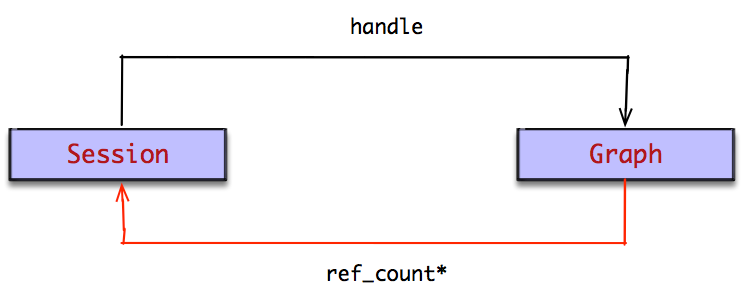
\includegraphics[width=0.7\textwidth]{figures/tf-graph-session-relation.png}
\caption{计算图:会话引用计数器技术}}
 \label{fig:tf-graph-session-relation}
\end{figure}

当需要删除图实例时,如果引用的\code{Session}数目为\ascii{0},则删除该图实例;否则,不删除图实例。

\begin{remark}
因此,之前实现操作\script{Session}的\ascii{C API}都被标识为已废弃(直至\ascii{1.2}版本还未删除),实现提供了一套新的\ascii{C API}管理\script{Session}的生命周期,以便改善系统的性能。
\end{remark}

\subsection{创建会话}

在\code{Session}创建时,在该图实例的\code{Session}数目加\ascii{1}。

\begin{leftbar}
\begin{c++}
TF_Session* TF_NewSession(TF_Graph* graph, const TF_SessionOptions* opt,
                          TF_Status* status) {
  Session* session;
  status->status = NewSession(opt->options, &session);
  if (status->status.ok()) {
    if (graph != nullptr) {
      mutex_lock l(graph->mu);
      graph->num_sessions += 1;
    }
    return new TF_Session(session, graph);
  } else {
    DCHECK_EQ(nullptr, session);
    return NULL;
  }
}
\end{c++}
\end{leftbar}

\subsection{销毁会话}

在\code{Session}销毁时,在该图实例的\code{Session}数目减\ascii{1}。

\begin{leftbar}
\begin{c++}
void TF_DeleteSession(TF_Session* s, TF_Status* status) {
  status->status = Status::OK();
  TF_Graph* const graph = s->graph;
  if (graph != nullptr) {
    graph->mu.lock();
    graph->num_sessions -= 1;
    const bool del = graph->delete_requested && graph->num_sessions == 0;
    graph->mu.unlock();
    if (del) delete graph;
  }
  delete s->session;
  delete s;
}
\end{c++}
\end{leftbar}

\subsection{删除图实例}

当需要删除图实例时,如果引用的\code{Session}数目为\ascii{0},则删除该图实例;否则,不删除该图实例。

\begin{leftbar}
\begin{c++}
void TF_DeleteGraph(TF_Graph* g) {
  g->mu.lock();
  g->delete_requested = true;
  const bool del = g->num_sessions == 0;
  g->mu.unlock();
  if (del) delete g;
}
\end{c++}
\end{leftbar}

\end{content}